\documentclass[a4paper,12pt]{article}

% --- Packages ---
\usepackage[margin=2.5cm]{geometry}
\usepackage{booktabs}
\usepackage{multirow}
\usepackage{caption}
\usepackage{lscape}
\usepackage{graphicx}
\usepackage{amsmath}
\usepackage{hyperref}
\usepackage{natbib}
\usepackage{setspace}
\onehalfspacing

% --- Title ---
\title{Spatial Structure Beyond the Power Spectrum: Amplitude-Adjusted Surrogate Testing in Natural and Synthetic Images}
\author{Scott Cundill\\Independent Researcher, Okinawa, Japan}
\date{}

\begin{document}
\maketitle

\begin{center}
\small DOI: \url{https://doi.org/10.5281/zenodo.20567808}
\end{center}

% =====================================================================
% ABSTRACT
% =====================================================================
\begin{abstract}
The Fourier power spectrum captures only second-order statistics of an image, leaving most spatial structure encoded in the phase. Standard phase-randomisation surrogates confound tests of phase-dependent structure because they also Gaussianize the amplitude distribution, producing an ambiguity: separation from surrogates could reflect spatial geometry or could reflect the shift from non-Gaussian to Gaussian, and the surrogate method itself cannot distinguish the two. This study applies iterative amplitude-adjusted Fourier transform (IAAFT) surrogates, which preserve both the power spectrum and the amplitude distribution, to a multi-metric image analysis pipeline spanning fractal, geometric, and topological measures. The method is validated against a non-Gaussian unstructured control image, with seventeen of eighteen metrics correctly registering no separation. Across six image categories drawn from three domains, human portraits photographic and AI-generated, coral reef tissue, and quasicrystalline materials, the results separate into two distinct layers. Fractal dimension, lacunarity, and junctions detect spatial structure near-universally, with large effect sizes regardless of image domain. Persistence homology metrics computed on edge-extracted point clouds detect a second, more specific layer, the closed-contour edge topology of biological and face images, present in faces of both photographic and synthetic origin, present in healthy coral, and largely absent in quasicrystal. Bilateral symmetry is shown to be substantially a frequency-domain property and does not separate under IAAFT. The two structural layers dissociate across categories, offering a more precise characterisation of spatial structure beyond the power spectrum than any single metric or null model can supply alone.
\end{abstract}

% =====================================================================
% 1. INTRODUCTION
% =====================================================================
\section{Introduction}

The Fourier power spectrum of an image captures its second-order statistics, the distribution of energy across spatial frequencies, but says nothing about how that energy is arranged in space. Two images with identical power spectra can be visually unrelated, one a coherent photograph, the other a noise field that happens to share the same frequency profile. Most of what makes an image recognisable, the edges and contours and geometric arrangements, lives in the Fourier phase rather than the amplitude \citep{oppenheim1981}. The question of how to measure phase-dependent structure has become central to image analysis across disciplines, from natural scene statistics and visual perception to materials characterisation, biological tissue imaging, and the recent surge of work on synthetic media.

The standard tool for testing whether a metric responds to phase structure is surrogate analysis. The technique was developed for nonlinear time series \citep{theiler1992} and extended to images by randomising the Fourier phase while preserving the amplitude spectrum. If a metric distinguishes an image from its phase-randomized surrogates, the inference is that the metric captures structure beyond the power spectrum. A large number of studies across image analysis, ecology, neuroscience, and materials science rely on this logic.

The logic has a hidden flaw, recognised in the nonlinear dynamics literature but rarely addressed in image work. Phase randomisation does not only destroy spatial structure, it also Gaussianizes the amplitude distribution, by the central limit theorem applied to the inverse Fourier transform of fixed amplitudes with uniformly randomised phases. Natural images are strongly non-Gaussian, with skewed and heavy-tailed intensity histograms shaped by scene content and acquisition processes. A metric that responds to non-Gaussianity, even partially, will register separation from phase surrogates whether or not it detects any spatial structure \citep{rapp1994}. The separation is real, but its interpretation is ambiguous, it could reflect spatial geometry, or it could reflect the distributional shift from skewed to Gaussian, and the surrogate method itself provides no way to distinguish the two.

A cleaner null model exists. The iterative amplitude-adjusted Fourier transform, introduced by \citet{schreiber1996}, generates surrogates that preserve both the power spectrum and the amplitude distribution, by iteratively swapping in the target spectrum amplitudes and rank-ordering pixel values against the target intensity distribution. The result is statistically indistinguishable from the original in both frequency content and intensity histogram, but with spatial phase structure destroyed. Any metric that separates an image from its IAAFT surrogates must be responding to phase-dependent structure, not to amplitude properties that the surrogate happens to alter. The method has been used in geophysics and neuroscience, and in some texture analysis work, but its systematic application to topological and geometric image metrics has not, to our knowledge, been previously reported.

This study applies IAAFT surrogate testing to a multi-metric, multi-domain image analysis pipeline. The metric set spans four broad classes, fractal and scaling metrics, geometric and morphological metrics, distributional metrics, and topological metrics derived from persistent homology on edge-extracted point clouds. The image dataset spans six categories across three domains, human portraits photographic and AI-generated, coral reef tissue healthy and bleached, and quasicrystalline materials at atomic resolution. The design tests, metric by metric and category by category, which aspects of image structure exceed the power spectrum and which do not. The same surrogate ensemble is applied to a non-Gaussian unstructured control image, providing direct empirical confirmation that any metric flagging the control as ``structured'' is responding to a confound rather than to spatial geometry.

The results fall into two layers. A near-universal layer, fractal dimension, lacunarity, and junctions, detects spatial structure consistently across all six categories with effect sizes large enough to leave little ambiguity. A category-dependent layer, persistent homology of edge contour topology, detects structure strongly in face images, moderately in healthy coral, and weakly or not at all in quasicrystal and bleached coral. The two layers are independent, they dissociate across categories, and together they describe spatial structure with a precision that no single metric or any single null model could achieve alone. The remainder of the paper sets out the method, the controls, the per-category results, and the implications for surrogate-based image analysis more broadly.

% =====================================================================
% 2. METHODS
% =====================================================================
\section{Methods}

\subsection{Metrics}

The analysis pipeline is implemented as SCOTT (Structural and Coherent Order in Topological Transforms), an open-source image analysis instrument. It computes a set of scalar metrics from each greyscale image, spanning four broad categories: fractal and scaling metrics (fractal dimension, lacunarity, multifractal width, multiscale entropy slope), geometric and morphological metrics (Euler characteristic mean, standard deviation, and range, junctions, clustering, orientation coherence, bilateral symmetry, plateau), distributional metrics (Shannon entropy), and topological metrics derived from persistent homology (Betti numbers, persistence entropy, total persistence). Full definitions and implementation details are available in the SCOTT project repository. A separate technical note \citep{cundill2026bokeh} demonstrates the framework on optical bokeh, detecting the central obstruction of a mirror lens as a persistent homology signature in 2D photographs.

The topological metrics require a specific construction. Each image is downsampled to a $64 \times 64$ pixel grid and Canny edge detection \citep{canny1986} is applied with fixed thresholds of 50 and 150. The coordinates of the resulting edge pixels form a two-dimensional point cloud, capped at 600 points via deterministic even-spaced subsampling when necessary. Ripser \citep{tralie2018} computes the Vietoris-Rips persistence diagrams of this cloud through homological dimension one. $H_0$ features correspond to connected clusters of edge points, and $H_1$ features correspond to closed curves traced by edge points in proximity, such as the contours surrounding eyes, polyp boundaries, or other enclosed edge geometry. Features with lifetimes below 5\% of the maximum finite death value are filtered as topological noise. The remaining features yield four scalar metrics: Betti-0 and Betti-1 (counts of persistent components and loops), persistence entropy of $H_1$ (the Shannon entropy of the normalised lifetime distribution, measuring how evenly distributed the loop structure is), and total persistence of $H_1$ (the sum of all loop lifetimes, measuring aggregate topological richness).

This construction means the $H_1$ metrics are sensitive to closed contour structure in the image's edge map, not to enclosed regions in the intensity field. The distinction matters: a face image produces closed edge contours around eyes, nostrils, and lips, and these form genuine loops in the Vietoris-Rips complex. A quasicrystal image, despite carrying strong spectral and fractal order, produces edge patterns that do not close into loops at comparable scales. The $64 \times 64$ downsampling and 600-point cap are deliberate speed-accuracy tradeoffs, documented and fixed across all images, ensuring that comparisons between originals and surrogates reflect structural differences rather than processing differences.

\subsection{Phase randomization and the Gaussianization confound}

Surrogate analysis is the standard test for whether a signal carries structure beyond its power spectrum, generating signals that share the original's power spectrum but lack its spatial structure \citep{theiler1992}. For images, the Fourier phase is randomized while the amplitude spectrum is preserved, producing surrogates with identical second-order statistics but destroyed spatial coherence \citep{oppenheim1981}. If a topological metric separates the original from its surrogates, the inference is that the metric responds to spatial structure, not frequency content.

The inference, however, rests on a critical flaw. Phase randomization does not only destroy spatial structure, it also Gaussianizes the pixel intensity distribution. The inverse Fourier transform of fixed amplitudes with uniformly randomized phases converges to Gaussian by the central limit theorem, regardless of the original. Natural images are strongly non-Gaussian, with intensity histograms showing skewness, heavy tails, and multimodal structure arising from scene content. Any metric sensitive to the amplitude distribution, even partially, will separate the original from its surrogates not because it detects spatial structure, but because it detects the shift from non-Gaussian to Gaussian \citep{rapp1994}.

If a topological metric separates a coral image from its phase surrogates, the separation may reflect the coral's non-Gaussian intensity profile, not its spatial geometry. Replication across images or categories does not resolve this, it is a flaw in the null model itself. A surrogate method that preserves both the power spectrum and the amplitude distribution isolates spatial structure as the sole variable, and the iterative amplitude-adjusted Fourier transform (IAAFT) does exactly this, described in Section~2.3.

\subsection{Iterative amplitude-adjusted Fourier transform surrogates}

The iterative amplitude-adjusted Fourier transform (IAAFT) method, introduced by \citet{schreiber1996}, resolves the Gaussianization confound by preserving both the power spectrum and the amplitude distribution of the original signal. The algorithm begins by storing two targets: the sorted pixel values of the original image, and the Fourier amplitude spectrum. Starting from a random shuffle of the original pixels, the procedure iterates: the current image is Fourier-transformed, its amplitudes are replaced with the target spectrum while phases are retained, the inverse transform is applied, and the resulting pixel values are rank-ordered and replaced with the stored target distribution. Each iteration refines the match to both targets simultaneously, and the process continues until convergence.

The result is a surrogate that is statistically indistinguishable from the original in both frequency content and intensity distribution, but whose spatial phase structure is randomized. The critical property, unlike phase-only surrogates, is that the amplitude distribution is preserved exactly, not approximately. For two-dimensional images, the algorithm extends directly by treating the 2D FFT amplitude spectrum as the target, and applying rank-order amplitude adjustment to the full pixel array. Our implementation runs at approximately 3.5 seconds per surrogate at $512 \times 512$ resolution, making ensemble generation computationally practical.

Verification confirmed that the method meets both preservation targets. Pixel intensity histograms of surrogates matched the originals with $L_1$ distance of zero, confirming exact amplitude preservation. Spectral power matched the target with mean squared error below 1\%, confirming near-exact frequency preservation. Entropy, a metric wholly determined by the amplitude distribution, registered zero separation across all twenty surrogates for every image in every category in this study, providing a continuous built-in validation that the method is functioning correctly throughout.

% --- FIGURE 1 ---
\begin{figure*}[ht]
\centering
\includegraphics[width=\textwidth]{figure_1_method_comparison.pdf}
\caption{Original images alongside phase-randomized and IAAFT surrogates. Left column: original images. Centre: phase surrogates, which Gaussianize the amplitude distribution (visible as contrast washout). Right: IAAFT surrogates, which preserve the amplitude distribution but destroy spatial phase structure. Top row: portrait face (FFHQ). Bottom row: quasicrystal (Mn--Cr--Ni--Si dodecagonal, Ishimasa).}
\label{fig:method_comparison}
\end{figure*}

\subsection{The non-Gaussian unstructured control}

Preserving the amplitude distribution removes the Gaussianization confound at the level of the null model, but it does not guarantee that every individual metric is clean. A metric could, in principle, respond to some other distributional artifact, or to subtle correlations introduced by the IAAFT iteration itself, rather than to genuine spatial structure. To test this directly, we constructed a non-Gaussian control image with no spatial structure: spatially independent pixels drawn from a gamma distribution (shape 2.0, scale 30.0), chosen to produce a representative heavy-tailed distribution; the specific parameter values are not critical to the control's purpose, as any non-Gaussian spatially independent image would serve. This produced a skewness of approximately 1.3 and a measured spatial autocorrelation below 0.005. The image is non-Gaussian by construction, but contains no spatial organisation, no edges, no clusters, no geometry.

We then generated twenty IAAFT surrogates of this control image and computed z-scores for every metric in the instrument. The logic is straightforward: if a metric separates the unstructured control from its surrogates, that metric is responding to something other than spatial structure, and must be excluded from any structural claims. If a metric does not separate, it is confirmed as structure-sensitive only. The results, reported in Section~3.2, identify one contaminated metric and validate the remainder.

\subsection{Datasets}

Six image categories were drawn from three domains: human faces, coral reef tissue, and quasicrystalline materials. The face domain comprised three categories: real portrait photographs from the FFHQ dataset \citep{karras2019}, AI-generated portraits from the Kaggle Real and Fake Faces dataset \citep{xhlulu2020}, and age-labelled photographs from the FG-NET facial aging dataset \citep{panis2016}. The coral domain comprised healthy and bleached reef specimens from a Flickr-sourced classification dataset of 923 images collected from Indonesian reef locations by multiple photographers \citep{muhammad2023}. Images were labelled by visual inspection as healthy (438) or bleached (485) and were not acquired under controlled survey conditions. The materials domain comprised three verified quasicrystal specimens provided directly by Prof.\ Tsutomu Ishimasa (Hokkaido University): two dodecagonal (12-fold) Mn--Cr--Ni--Si images and one icosahedral (5-fold) Zn--Mg--Ho image. For each large-pool category, thirty images were sampled at random with a fixed seed. Quasicrystal specimens were used in full.

The three domains were selected to span image formation processes as different as possible: photographs of biological subjects, microscopic tissue surveys, and atomic-resolution electron micrographs. Greyscale conversion was applied to ensure consistent treatment across domains where colour carries different meaning and is not always available, and normalisation removed contrast differences that would otherwise confound surrogate ensembles. No further domain-specific preprocessing was applied. The diversity of image sources is deliberate, the paper's central claim concerns structure detection across image types rather than within any single category.

\subsection{Statistical procedure}

For each image, twenty IAAFT surrogates were generated and the full metric set was computed on the original and on each surrogate. A per-image z-score was calculated as:
\begin{equation}
z = \frac{x_{\text{orig}} - \mu_{\text{surr}}}{\sigma_{\text{surr}}}
\end{equation}
where $x_{\text{orig}}$ is the metric value on the original image, and $\mu_{\text{surr}}$ and $\sigma_{\text{surr}}$ are the mean and standard deviation across the twenty surrogates. A metric was classed as separated for that image if the absolute z-score exceeded 2.0, corresponding approximately to a two-tailed $p$-value of 0.05 under normality. The separation rate for a category was then the proportion of images in that category meeting this criterion, and the mean absolute z-score served as a proxy for effect size. Both quantities are reported throughout the results. The analysis is exploratory across multiple metrics and categories, and z-scores are reported as heuristic screens rather than confirmatory tests.

Two edge cases were handled consistently. Where surrogate standard deviation was zero, the z-score was undefined and the image was excluded from the separation rate for that metric, with the count of valid images noted. This affected the forbidden\_coverage metric in a small number of images, where all twenty surrogates produced identical zero values, and results for that metric are reported qualitatively rather than as z-scores. The orientation\_coherence metric, though producing large z-scores across all categories, was flagged during the non-Gaussian control experiment as separating unstructured noise from its surrogates, and is reported throughout with a contamination caveat.

% =====================================================================
% 3. RESULTS
% =====================================================================
\section{Results}

\subsection{IAAFT verification}

Surrogates were verified against both preservation targets before the main experiment. Pixel intensity histograms matched the originals with an $L_1$ distance of zero across all test images, confirming exact amplitude preservation. Fourier power spectra matched the target with a mean squared error below 1\%, confirming near-exact frequency preservation. These two properties together define a valid IAAFT surrogate, and both were met.

The entropy metric provided a continuous in-experiment validation throughout the main results. Entropy is a function of the amplitude distribution only, carrying no spatial information, and registered zero separation across all twenty surrogates for every image in every category. This is the expected result if the method is preserving the amplitude distribution correctly, and the consistency of this result across 154 images and six categories confirms the method was functioning as intended throughout.

\subsection{The non-Gaussian unstructured control}

Twenty IAAFT surrogates of the non-Gaussian unstructured noise image were generated and the full metric set computed. Seventeen of eighteen metrics showed no separation, with absolute z-scores below 1.0 in all but one case. Fractal dimension, lacunarity, all Euler metrics, all persistence homology metrics, junctions, clustering, and multiscale entropy slope were indistinguishable from their surrogates, confirming that none of these metrics responds to a non-Gaussian amplitude distribution in the absence of spatial structure. The entropy metric registered zero separation, as expected.

One metric separated: orientation\_coherence, with a z-score of 3.44. This indicates the metric retains some sensitivity to distributional properties beyond spatial phase structure, and it is flagged as contaminated for the remainder of this study. Results for orientation\_coherence are reported in full throughout, but are excluded from any structural claims. The remaining seventeen metrics are treated as validated structure-sensitive instruments, and results from Section~3.3 onwards apply to these only.

% --- FIGURE 2 ---
\begin{figure*}[ht]
\centering
\includegraphics[width=0.75\textwidth]{figure_2_control.pdf}
\caption{The non-Gaussian unstructured control. Left column: gamma-distributed noise with no spatial structure. Right column: a real face image with genuine spatial structure. Top row: originals. Middle row: IAAFT surrogates. Bottom row: absolute pixel difference (enhanced $4\times$). The noise surrogate is visually indistinguishable from the original (uniform difference map), while the face surrogate shows clear destruction of spatial structure (face contours visible in the difference map). This confirms that IAAFT separation reflects spatial structure, not distributional properties.}
\label{fig:control}
\end{figure*}

\subsection{Near-universal structure detectors}

Three metrics separated the original from its IAAFT surrogates consistently across all six categories. Fractal dimension achieved separation rates of 83--100\% in the five large-pool categories, with mean absolute z-scores ranging from 19 to 70, and 67\% in quasicrystal. Lacunarity followed the same pattern, with separation rates of 87--100\% in the five large categories and 67\% in quasicrystal. Junctions achieved separation rates of 80--100\% across all six categories, including quasicrystal, making it the only metric to clear the 80\% threshold in every category. Z-scores for all three metrics were large throughout, ranging from 7 to 70, well above the threshold at which borderline interpretations apply.

The lower separation rates for fractal dimension and lacunarity in the quasicrystal category are most plausibly a statistical power effect. With $n = 3$ valid images, separation rates should be read as indicative rather than definitive, though the mean z-scores of 13.6 and 16.2 are among the largest seen across all categories, indicating the effect is present and substantial. The FG-NET category also showed modestly lower rates for both metrics (67\% and 70\%), consistent with the greater photographic heterogeneity of that dataset, which spans several decades of age and varied imaging conditions.

In every category, real images had lower fractal dimensions than their surrogates, and higher lacunarity. This is the expected signature of spatial structure: genuine images are less space-filling, and more gapped, than phase-randomized versions of themselves at the same power spectrum. The effect is not subtle. It persists across portrait photography, coral reef microscopy, and atomic-resolution electron micrographs, across image sizes from tens of pixels to thousands, and across the full range of image content represented in this dataset.

% --- TABLE 1 (inline) ---
\begin{landscape}
\begin{table}[ht]
\centering
\small
\caption{IAAFT surrogate separation rates (Sep\%) and mean absolute z-scores (mean$|z|$) for each metric across six image categories. Each cell shows Sep\% / mean$|z|$. Values $\geq$80\% in Sep\% are \textbf{bold}. $n = 30$ images per large-pool category; $n = 3$ for quasicrystal (QC); 20 IAAFT surrogates per image. $^\dagger$\,Orientation coherence separated the non-Gaussian unstructured control (Section~2.4) and is excluded from structural claims.}
\label{tab:results}
\begin{tabular}{llcccccc}
\toprule
& & \multicolumn{6}{c}{\textbf{Image category}} \\
\cmidrule(lr){3-8}
\textbf{Metric} & \textbf{Group} & \textbf{AI Faces} & \textbf{Real Faces} & \textbf{FG-NET} & \textbf{Coral (H)} & \textbf{Coral (B)} & \textbf{QC} \\
\midrule
\multicolumn{8}{l}{\textit{Near-universal structure detectors}} \\[2pt]
Fractal dimension & Universal & \textbf{100\%}/23.9 & \textbf{97\%}/25.3 & 67\%/19.1 & \textbf{87\%}/69.6 & \textbf{83\%}/27.6 & 67\%/13.6 \\
Lacunarity & Universal & \textbf{100\%}/39.7 & \textbf{97\%}/42.5 & 70\%/68.6 & \textbf{93\%}/69.5 & \textbf{87\%}/31.5 & 67\%/16.2 \\
Junctions & Universal & \textbf{100\%}/16.8 & \textbf{100\%}/15.6 & \textbf{97\%}/7.7 & \textbf{93\%}/8.3 & \textbf{80\%}/7.4 & \textbf{100\%}/12.9 \\
\midrule
\multicolumn{8}{l}{\textit{Geometric metrics}} \\[2pt]
MS entropy slope & Geometric & 70\%/6.1 & 70\%/6.0 & \textbf{87\%}/6.4 & 30\%/3.0 & 23\%/2.0 & 33\%/2.4 \\
Euler std & Geometric & 60\%/4.6 & 77\%/6.1 & 53\%/4.0 & \textbf{87\%}/8.2 & 70\%/7.5 & 67\%/4.2 \\
Euler range & Geometric & 37\%/2.7 & 50\%/3.2 & 50\%/3.5 & \textbf{80\%}/4.8 & 57\%/4.4 & 33\%/2.1 \\
Clustering & Geometric & 33\%/2.6 & 37\%/2.6 & 10\%/1.4 & 7\%/1.5 & 37\%/2.1 & \textbf{100\%}/8.3 \\
\midrule
\multicolumn{8}{l}{\textit{Topological metrics (persistent homology, $H_1$)}} \\[2pt]
Betti-1 & TDA & 57\%/3.7 & 67\%/3.4 & 37\%/2.7 & 43\%/3.3 & 23\%/2.1 & 33\%/2.4 \\
Persistence entropy & TDA & \textbf{80\%}/5.8 & 77\%/5.3 & 63\%/4.9 & 47\%/3.1 & 23\%/2.3 & 33\%/1.8 \\
Total persistence & TDA & \textbf{80\%}/5.0 & 70\%/4.6 & 60\%/3.6 & 57\%/3.8 & 23\%/2.3 & 67\%/2.9 \\
Betti-0 & TDA & 0\%/0.0 & 0\%/0.0 & 11\%/1.1 & 3\%/0.4 & 0\%/0.0 & 0\%/0.5 \\
\midrule
\multicolumn{8}{l}{\textit{Non-separating and validation metrics}} \\[2pt]
Bilateral symmetry & Non-sep & 20\%/2.1 & 30\%/2.5 & 20\%/2.2 & 10\%/1.5 & 7\%/1.3 & 33\%/2.6 \\
Entropy & Validation & 0\%/0.0 & 0\%/0.0 & 0\%/0.0 & 0\%/0.0 & 0\%/0.0 & 0\%/0.0 \\
\midrule
\multicolumn{8}{l}{\textit{Contaminated metric (reported for completeness only)}} \\[2pt]
Orient.\ coherence$^\dagger$ & Contam. & \textbf{100\%}/50.5 & \textbf{100\%}/60.6 & \textbf{80\%}/12.2 & \textbf{100\%}/45.0 & \textbf{100\%}/27.2 & \textbf{100\%}/14.2 \\
\bottomrule
\end{tabular}
\end{table}
\end{landscape}

\subsection{Category-dependent topological complexity}

Persistence homology metrics, specifically those derived from $H_1$ (one-dimensional topological features, the loops in the Vietoris-Rips complex of the edge point cloud), showed a markedly different pattern from fractal dimension and lacunarity, separating strongly in some categories and weakly in others. For AI-generated and real portrait faces, persistence entropy achieved separation rates of 80\% and 77\% respectively, with mean z-scores of 5.8 and 5.3, and total persistence followed at 80\% and 70\%. For FG-NET photographs, separation rates were somewhat lower, 63\% for persistence entropy and 60\% for total persistence, consistent with greater photographic heterogeneity. Healthy coral achieved 47\% for persistence entropy and 57\% for total persistence. Bleached coral and quasicrystal were largely non-separating, with rates of 23\% or below for all three TDA metrics. Betti-1 followed the same gradient, strongest in faces, weaker in healthy coral, near-zero in bleached coral and quasicrystal.

The pattern is consistent with the edge geometry of each image type. Faces produce closed edge contours around eyes, nostrils, lips, and ear boundaries, forming genuine loops in the Vietoris-Rips complex that are destroyed when spatial phase structure is randomised. Healthy coral polyps produce similar closed-contour edge geometry at the microscopic scale, generating detectable loop structure in the original that surrogates lack. Quasicrystal images, despite carrying strong spectral and fractal structure, produce edge patterns that do not close into loops at comparable scales, and the persistence metrics respond accordingly. The separation gradient across categories reflects biological contour geometry, not image quality or dataset size.

The contrast between healthy and bleached coral warrants cautious interpretation. Healthy coral separated at 47--57\% on persistence entropy and total persistence, bleached coral at 23\% on both. However, the two groups were drawn from a compiled classification dataset sourced from multiple photographers, locations, and imaging conditions, and the difference in TDA separation rates may reflect acquisition variability rather than biological structure. Both groups produced strong separation on fractal dimension and lacunarity, confirming that coral images of both types carry spatial structure beyond the power spectrum. Whether the TDA difference tracks biological state specifically requires a dataset with controlled acquisition conditions and is not established by this study.

% --- FIGURE 3 ---
\begin{figure*}[ht]
\centering
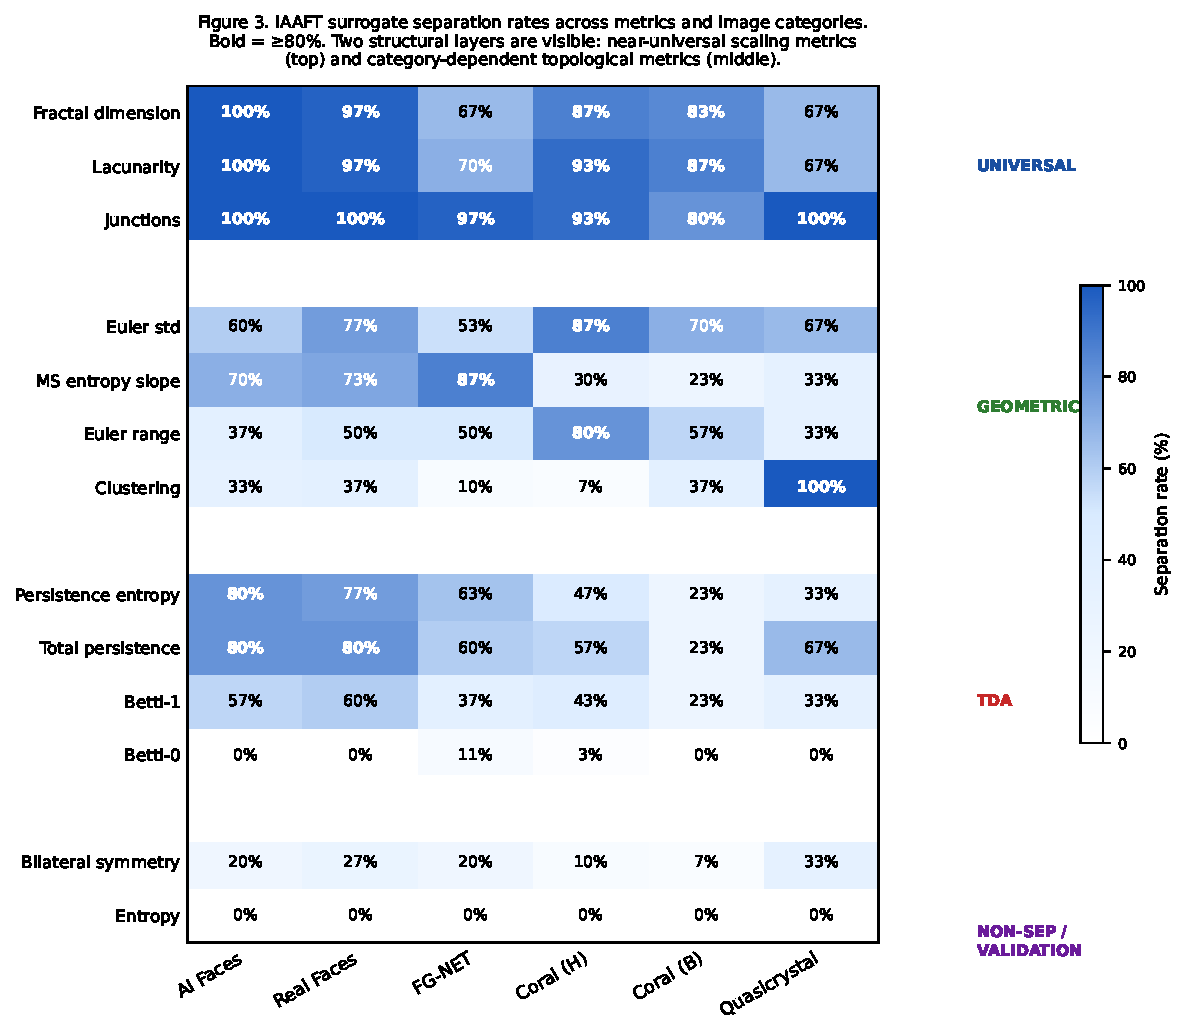
\includegraphics[width=\textwidth]{figure_3_heatmap.pdf}
\caption{IAAFT surrogate separation rates across metrics and image categories. Each cell shows the percentage of images with $|z| > 2.0$. Bold values indicate $\geq$80\% separation. Two structural layers are visible: near-universal scaling metrics (fractal dimension, lacunarity, junctions) at top, and category-dependent topological metrics (persistence entropy, total persistence, Betti-1) in the middle section. Entropy (bottom row) shows 0\% separation throughout, confirming the IAAFT method preserves the amplitude distribution.}
\label{fig:heatmap}
\end{figure*}

\subsection{Non-separating metrics and what they reveal}

Three metrics registered zero separation across all six categories: entropy, Betti-0, and tau\_ratio\_score. For entropy and Betti-0, this is the expected result. Entropy is determined entirely by the amplitude distribution, which IAAFT preserves exactly, and its consistent zero separation throughout the experiment confirms the method was functioning correctly in every image and every category. Betti-0 counts connected components in the thresholded image, a property stable under phase randomisation at the scales used here. These metrics are non-separating by design, and their behaviour confirms the null model is sound.

Bilateral symmetry produced separation rates of 7--30\% across categories, consistently weak, and showed no meaningful separation in most images. This is not a failure of the metric, it is a property of what bilateral symmetry measures. A bilaterally symmetric image has a power spectrum that reflects that symmetry, and because IAAFT preserves the power spectrum, surrogates tend to inherit bilateral structure from the original. Bilateral symmetry is largely a frequency-domain property, detectable in the second-order statistics of the image rather than in its spatial phase structure. This is consistent with the finding in a companion study \citep{cundill2026bilateral} that bilateral symmetry strongly discriminates between image categories at the population level, as a category-level property, while not separating individual images from their phase-matched surrogates. Multifractal width followed a similar pattern, with separation rates of 10--33\% and no consistent signal across categories.

% =====================================================================
% 4. DISCUSSION
% =====================================================================
\section{Discussion}

\subsection{What IAAFT surrogates establish}

Phase-randomized surrogates have been widely used to test for structure in image data, but the Gaussianization confound means that any separation found with phase surrogates is ambiguous, it could reflect genuine spatial structure or it could reflect the distributional shift from non-Gaussian to Gaussian. This ambiguity cannot be resolved by replication, by larger sample sizes, or by choosing metrics carefully. It is a property of the null model, and it applies to every metric applied to every image regardless of domain. IAAFT surrogates remove this ambiguity by construction, preserving the amplitude distribution exactly, so that any remaining separation must reflect phase-dependent spatial structure.

The non-Gaussian unstructured control provides the empirical confirmation. Seventeen of eighteen metrics failed to separate non-Gaussian noise from its IAAFT surrogates, confirming that those metrics do not respond to distributional properties in the absence of spatial structure. The combination of a distributional-preserving null model and a structured null-hypothesis test converts a previously ambiguous result into a clean one: separation now means structure, not distribution. The results in Sections~3.3 and 3.4 are interpretable in that direct sense, across all six categories and across metrics as different as fractal dimension and persistence entropy.

\subsection{Two layers of structure}

The results separate into two distinct layers. The first is near-universal, fractal dimension, lacunarity, and junctions separated consistently across all six categories, with large z-scores and high separation rates regardless of image domain. These metrics respond to properties present in every structured image tested, the relative sparsity of real images compared to their surrogates, the gap structure of natural scenes and biological tissue and crystalline materials alike. The second layer is category-dependent, persistence homology metrics separated strongly in face images, moderately in healthy coral, and weakly or not at all in bleached coral and quasicrystal. These metrics respond to something present in some structured images but not others.

The distinction maps onto a meaningful physical difference. Fractal dimension and lacunarity measure scaling properties, present wherever spatial organisation exists at multiple scales, which includes every image category tested. Persistence homology, specifically $H_1$, measures closed curves in the edge structure that persist across a range of distance thresholds. Faces and healthy coral produce recurring closed edge contours, the boundaries of eyes, nostrils, coral polyps, and IAAFT destroys the spatial phase relationships that generate these contour patterns. Notably, the topological signature was as strong in AI-generated portraits as in photographic ones, indicating that the generative model used to produce them reproduces this aspect of face geometry alongside its other features. Quasicrystal images carry strong spectral and fractal organisation, but their edge maps do not form closed loops at comparable scales. The two layers are not in competition, they are measuring genuinely different aspects of spatial structure, and the fact that they dissociate across categories is itself informative about the nature of the image types.

\subsection{The coral provenance caveat}

The coral categories illustrate both the strength and the limits of the surrogate approach. Both healthy and bleached coral produced strong, consistent separation on fractal dimension, lacunarity, and junctions, confirming that coral reef images carry spatial structure beyond the power spectrum regardless of reef health state. The universal metrics, responding to scaling and morphological properties common to most natural imagery, are inherently less sensitive to acquisition variation than the contour-specific topological metrics, and their consistent separation across both coral groups is reassuring on this front. TDA separation rates differed between the two groups, but the coral dataset was compiled from multiple public sources without controlled acquisition conditions, and this study cannot distinguish a biological effect from an imaging confound. A direct check of mean brightness found only 5.8 units difference (out of 255) between healthy and bleached groups, with fully overlapping standard deviations, suggesting that gross exposure differences are unlikely to drive the TDA separation, though subtler acquisition confounds cannot be excluded. Resolving this would require a coral dataset acquired under uniform survey conditions, with both health states imaged by the same equipment at comparable depths, and represents a natural next step for this line of work.

\subsection{Bilateral symmetry as a frequency-domain property}

Bilateral symmetry produced separation rates of 7--30\% across all six categories, consistently weak, and the pattern warrants interpretation rather than dismissal. A bilaterally symmetric image has a power spectrum that encodes that symmetry, the amplitude spectrum of a left-right symmetric image carries the same left-right relationship as the image itself, and IAAFT surrogates, preserving the amplitude spectrum exactly, tend to inherit this property. The metric measures something real, it strongly discriminates between image categories at the population level \citep{cundill2026bilateral}, but the information it carries is largely accessible in the second-order statistics of the image. Phase randomisation, even without amplitude adjustment, largely preserves it.

This places bilateral symmetry in a different class from fractal dimension, lacunarity, and persistence homology. Those metrics detect structure that exists in the spatial phase relationships of an image, structure that IAAFT destroys. Bilateral symmetry, in large part, does not. Recognising this distinction is practically useful, bilateral symmetry is a valid and powerful descriptor for comparing image populations, but it is not evidence of spatial structure beyond the power spectrum, and should not be interpreted as such in surrogate-based analyses.

\subsection{Limitations}

The quasicrystal category comprised three unique images, a constraint of specimen availability rather than experimental design, and separation rates for that category should be read as indicative rather than definitive. The near-universal separators, fractal dimension, lacunarity, and junctions, all produced z-scores in the range of 12--16 for quasicrystal despite the 67--100\% separation rates, suggesting the effect is present and the z-scores are substantial given the small sample. One metric, orientation\_coherence, was excluded from structural claims after separating the non-Gaussian unstructured control, and its results are reported throughout for completeness but carry a contamination caveat. The forbidden\_coverage metric produced undefined z-scores for a small number of images where all surrogates returned zero values, and is reported qualitatively in those cases.

The non-Gaussian control used a gamma-distributed noise image with spatial independence. This tests one class of non-Gaussian structure, the most direct threat to the Rapp critique, but does not exhaust all possible confounds. Images with spatially correlated non-Gaussian noise, or with non-stationarity in the amplitude distribution, could in principle produce separation under IAAFT for reasons other than spatial phase structure, and this study does not test those cases. All images were analysed in greyscale, and colour-channel structure, where present, was not examined. The coral dataset was compiled from publicly available images of unknown and likely heterogeneous provenance, and comparisons between the healthy and bleached categories should be treated as observational rather than controlled. The AI-generated portrait category used StyleGAN-derived images, and the synthetic media landscape has shifted toward diffusion and flow-based architectures that may produce different spatial phase signatures, so the topological findings for AI faces should not be generalised to all classes of generative model without further testing. The category-dependent TDA findings rest on within-category comparisons of images against their own surrogates, not direct between-category comparisons, and inferences about cross-category differences in topological complexity should be drawn with that design in mind.

% =====================================================================
% 5. CONCLUSION
% =====================================================================
\section{Conclusion}

Topological and geometric metrics of natural images carry spatial structure that their power spectra cannot account for. This study demonstrates that claim rigorously, using amplitude-adjusted surrogates that preserve both the frequency content and the intensity distribution of each image, and verifying metric-by-metric that separation reflects spatial phase structure rather than distributional properties. The method is reproducible, computationally practical, and the validation framework is built into the experiment itself, with entropy as a continuous null check throughout.

The findings divide cleanly into two layers. Fractal dimension, lacunarity, and junctions detect structure near-universally, across portrait photography, coral reef microscopy, and atomic-resolution electron micrographs, with z-scores large enough to leave little ambiguity. Persistence homology metrics detect a second, more specific layer, the closed-contour edge topology of biological and face images, present in faces of both photographic and synthetic origin, present in healthy coral, reduced in bleached coral, and largely absent in quasicrystal. These two layers are independent, they dissociate across categories, and together they describe a richer picture of spatial structure than either could provide alone.

% =====================================================================
% BACK MATTER
% =====================================================================

\section*{Data and code availability}
All code used in this study, including the IAAFT implementation, the metric pipeline, and the surrogate analysis scripts, is available in the SCOTT project repository at \url{https://github.com/scottcundill/scott-framework}. Raw image datasets are publicly available from their respective sources as cited. Quasicrystal specimens beyond the published image are available from Prof.\ Tsutomu Ishimasa upon reasonable request. The complete set of per-image z-scores, separation rates, and surrogate analysis outputs is included in the repository as CSV files.

\subsection*{How to cite this work}

\begin{quote}
Cundill, S. (2026). Spatial Structure Beyond the Power Spectrum:
Amplitude-Adjusted Surrogate Testing in Natural and Synthetic Images. Zenodo.
\url{https://doi.org/10.5281/zenodo.20567808}
\end{quote}

\section*{Acknowledgments}
The author thanks Prof.\ Tsutomu Ishimasa (Hokkaido University) for providing the quasicrystal specimens that anchor the materials category of this study.

\section*{Author contributions}
S.C.\ designed the study, implemented the pipeline, performed the experiments, analysed the data, and wrote the manuscript.

\section*{Funding}
This work received no external funding.

\section*{Competing interests}
The author declares no competing interests.

\section*{AI use disclosure}
AI language models including Claude (Anthropic), Gemini (Google), ChatGPT (OpenAI), and Grok (xAI) were used in code development, data analysis, and manuscript preparation.

% ── References ────────────────────────────────────────────────────────────────
\bibliographystyle{plainnat}

\begin{thebibliography}{99}

\bibitem[Canny(1986)]{canny1986}
Canny, J. (1986).
\newblock A computational approach to edge detection.
\newblock \textit{IEEE Transactions on Pattern Analysis and Machine
Intelligence}, PAMI-8(6), 679--698.
\newblock DOI: 10.1109/TPAMI.1986.4767851

\bibitem[Cundill(2026a)]{cundill2026bilateral}
Cundill, S. (2026).
\newblock Bilateral Symmetry as a Filter-Robust Discriminator Between Real and
GAN-Generated Face Images.
\newblock Zenodo. \url{https://doi.org/10.5281/zenodo.20567680}

\bibitem[Cundill(2026b)]{cundill2026bokeh}
Cundill, S. (2026).
\newblock Mirror Lens Central Obstruction Detected as Persistent Homology
Signature in 2D Photographs.
\newblock Technical Note. Zenodo. \url{https://doi.org/10.5281/zenodo.20564619}

\bibitem[Karras et~al.(2019)]{karras2019}
Karras, T., Laine, S., \& Aila, T. (2019).
\newblock A style-based generator architecture for generative adversarial
networks.
\newblock \textit{Proceedings of the IEEE/CVF Conference on Computer Vision and
Pattern Recognition (CVPR)}, pp.\ 4401--4410.
\newblock DOI: 10.1109/CVPR.2019.00453

\bibitem[Muhammad et~al.(2023)]{muhammad2023}
Muhammad, F., Elfandra, A.~B., Amin, I.~P., \& Wicaksono, A.~F. (2023).
\newblock Pengembangan model untuk mendeteksi kerusakan pada terumbu karang
dengan klasifikasi citra.
\newblock Dataset available at
\url{https://www.kaggle.com/datasets/vencerlanz09/healthy-and-bleached-corals-image-classification}

\bibitem[Oppenheim \& Lim(1981)]{oppenheim1981}
Oppenheim, A.~V. \& Lim, J.~S. (1981).
\newblock The importance of phase in signals.
\newblock \textit{Proceedings of the IEEE}, 69(5), 529--541.
\newblock DOI: 10.1109/PROC.1981.12022

\bibitem[Panis et~al.(2016)]{panis2016}
Panis, G., Lanitis, A., Tsapatsoulis, N., \& Cootes, T.~F. (2016).
\newblock Overview of research on facial ageing using the {FG-NET} ageing
database.
\newblock \textit{IET Biometrics}, 5(2), 37--46.
\newblock DOI: 10.1049/iet-bmt.2014.0053

\bibitem[Rapp et~al.(1994)]{rapp1994}
Rapp, P.~E., Albano, A.~M., Zimmerman, I.~D., \& Jim\'enez-Monta\~no, M.~A.
(1994).
\newblock Phase-randomized surrogates can produce spurious identifications of
non-random structure.
\newblock \textit{Physics Letters A}, 192(1), 27--33.
\newblock DOI: 10.1016/0375-9601(94)91010-3

\bibitem[Schreiber \& Schmitz(1996)]{schreiber1996}
Schreiber, T. \& Schmitz, A. (1996).
\newblock Improved surrogate data for nonlinearity tests.
\newblock \textit{Physical Review Letters}, 77(4), 635--638.
\newblock DOI: 10.1103/PhysRevLett.77.635

\bibitem[Theiler et~al.(1992)]{theiler1992}
Theiler, J., Eubank, S., Longtin, A., Galdrikian, B., \& Farmer, J.~D.
(1992).
\newblock Testing for nonlinearity in time series: the method of surrogate
data.
\newblock \textit{Physica D: Nonlinear Phenomena}, 58(1--4), 77--94.
\newblock DOI: 10.1016/0167-2789(92)90102-S

\bibitem[Tralie et~al.(2018)]{tralie2018}
Tralie, C., Saul, N., \& Bar-On, R. (2018).
\newblock Ripser.py: A lean persistent homology library for {Python}.
\newblock \textit{Journal of Open Source Software}, 3(29), 925.
\newblock DOI: 10.21105/joss.00925

\bibitem[xhlulu(2020)]{xhlulu2020}
xhlulu (2020).
\newblock 140k Real and Fake Faces.
\newblock Kaggle. \url{https://www.kaggle.com/datasets/xhlulu/140k-real-and-fake-faces}

\end{thebibliography}

\end{document}
